\documentclass{beamer}\usepackage[]{graphicx}\usepackage[]{color}
%% maxwidth is the original width if it is less than linewidth
%% otherwise use linewidth (to make sure the graphics do not exceed the margin)
\makeatletter
\def\maxwidth{ %
  \ifdim\Gin@nat@width>\linewidth
    \linewidth
  \else
    \Gin@nat@width
  \fi
}
\makeatother

\definecolor{fgcolor}{rgb}{1, 0.894, 0.769}
\newcommand{\hlnum}[1]{\textcolor[rgb]{0.824,0.412,0.118}{#1}}%
\newcommand{\hlstr}[1]{\textcolor[rgb]{1,0.894,0.71}{#1}}%
\newcommand{\hlcom}[1]{\textcolor[rgb]{0.824,0.706,0.549}{#1}}%
\newcommand{\hlopt}[1]{\textcolor[rgb]{1,0.894,0.769}{#1}}%
\newcommand{\hlstd}[1]{\textcolor[rgb]{1,0.894,0.769}{#1}}%
\newcommand{\hlkwa}[1]{\textcolor[rgb]{0.941,0.902,0.549}{#1}}%
\newcommand{\hlkwb}[1]{\textcolor[rgb]{0.804,0.776,0.451}{#1}}%
\newcommand{\hlkwc}[1]{\textcolor[rgb]{0.78,0.941,0.545}{#1}}%
\newcommand{\hlkwd}[1]{\textcolor[rgb]{1,0.78,0.769}{#1}}%
\let\hlipl\hlkwb

\usepackage{framed}
\makeatletter
\newenvironment{kframe}{%
 \def\at@end@of@kframe{}%
 \ifinner\ifhmode%
  \def\at@end@of@kframe{\end{minipage}}%
  \begin{minipage}{\columnwidth}%
 \fi\fi%
 \def\FrameCommand##1{\hskip\@totalleftmargin \hskip-\fboxsep
 \colorbox{shadecolor}{##1}\hskip-\fboxsep
     % There is no \\@totalrightmargin, so:
     \hskip-\linewidth \hskip-\@totalleftmargin \hskip\columnwidth}%
 \MakeFramed {\advance\hsize-\width
   \@totalleftmargin\z@ \linewidth\hsize
   \@setminipage}}%
 {\par\unskip\endMakeFramed%
 \at@end@of@kframe}
\makeatother

\definecolor{shadecolor}{rgb}{.97, .97, .97}
\definecolor{messagecolor}{rgb}{0, 0, 0}
\definecolor{warningcolor}{rgb}{1, 0, 1}
\definecolor{errorcolor}{rgb}{1, 0, 0}
\newenvironment{knitrout}{}{} % an empty environment to be redefined in TeX

\usepackage{alltt}
\usepackage{../371g-slides}
\title{Multiple Regression 2}
\subtitle{Lecture 13}
\author{STA 371G}
\IfFileExists{upquote.sty}{\usepackage{upquote}}{}
\begin{document}
  
  
  

  \frame{\maketitle}

  % Show outline at beginning of each section
  \AtBeginSection[]{
    \begin{frame}<beamer>
      \tableofcontents[currentsection]
    \end{frame}
  }

  %%%%%%% Slides start here %%%%%%%

  \begin{darkframes}
    \begin{frame}{Midterm 1 results}
      \begin{itemize}[<+->]
        \item Scores and feedback will be available in Canvas/Quest later today or tomorrow
        \item Approximately: mean = 74\%, median = 75\%, SD = 15\%
        \item Since this was our first exam using Quest, you can retake the exam and get up to half credit back starting Thursday 5 PM
        \item Example: if you got a 60\%, and you get a 100\% on the retake, your new Midterm 1 score will be 80\%
        \item Your retake submission is due one week later (Thursday, March 8 at 5 PM)
      \end{itemize}
      \note{Start with an LC Q2 to review}
    \end{frame}

    \begin{frame}[fragile]{Predicting median house prices in Boston}
\begin{knitrout}
\definecolor{shadecolor}{rgb}{0.137, 0.137, 0.137}\begin{kframe}
\begin{alltt}
\hlstd{> }\hlstd{model} \hlkwb{<-} \hlkwd{lm}\hlstd{(MEDV} \hlopt{~} \hlstd{CRIME} \hlopt{+} \hlstd{ZONE} \hlopt{+} \hlstd{NOX} \hlopt{+} \hlstd{ROOM} \hlopt{+} \hlstd{DIST}
\hlstd{+ }             \hlopt{+} \hlstd{RADIAL} \hlopt{+} \hlstd{TAX} \hlopt{+} \hlstd{PTRATIO} \hlopt{+} \hlstd{LSTAT,}
\hlstd{+ }             \hlkwc{data}\hlstd{=boston)}
\end{alltt}
\end{kframe}
\end{knitrout}
      \begin{columns}[onlytextwidth]
        \column{.5\textwidth}
          \begin{itemize}
            \item MEDV: Median Price (response)
            \item CRIME: Per capita crime rate
            \item ZONE: Proportion of large lots
            \item NOX: Nitrogen Oxide concentration
            \item DIST: Distance to employment centers
          \end{itemize}
        \column{.5\textwidth}
          \begin{itemize}
            \item ROOM: Average \# of rooms
            \item RADIAL: Accessibility to highways
            \item TAX: Tax rate (per \$10K)
            \item PTRATIO: Pupil-to-teacher ratio
            \item LSTAT: Proportion of ``lower status''
            %  proportion of adults without some high school education or that are classified as laborers
          \end{itemize}
      \end{columns}
    \end{frame}



    \begin{frame}[fragile]{Overall Null Hypothesis}
      Is our model useful? Let's look at $R^2$:
\begin{knitrout}
\definecolor{shadecolor}{rgb}{0.137, 0.137, 0.137}\begin{kframe}
\begin{alltt}
\hlstd{> }\hlkwd{summary}\hlstd{(model)}\hlopt{$}\hlstd{r.squared}
\end{alltt}
\begin{verbatim}
[1] 0.7282911
\end{verbatim}
\end{kframe}
\end{knitrout}
      \pause
      Can we be confident that our model will generalize to the \alert{population}?  \pause

      \bigskip

      $H_0: \beta_1=\beta_2=\beta_3=\beta_4=\beta_5=\beta_6=\beta_7=\beta_8=\beta_9=0$ (Data explains nothing!) \pause

      $H_A: \beta_i \neq 0$ for some $i$ (At least one predictor is useful) \pause

      or

      $H_0: R^2=0 \qquad H_A: R^2>0$
    \end{frame}



   \begin{frame}[fragile]{Overall Null Hypothesis}
      Check the $p$-value in the summary:
      \begin{center}
        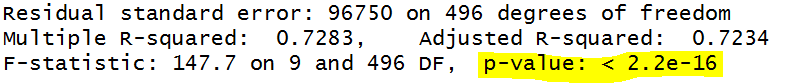
\includegraphics[width=4in]{r_sq_pval} \\
      \end{center}
      So we can reject the overall null hypothesis! \pause
      \bigskip
      ($R^2$ was already too big to suspect that it was actually zero in the population---and we already knew some predictors are statistically significant!)
    \end{frame}



    \begin{frame}[fragile]{How good are our predictions?}
      Let's plot the residuals (the discrepancies between the predicted and actual home prices). \pause

\begin{knitrout}
\definecolor{shadecolor}{rgb}{0.137, 0.137, 0.137}\begin{kframe}
\begin{alltt}
\hlstd{> }\hlkwd{hist}\hlstd{(}\hlkwd{resid}\hlstd{(model),} \hlkwc{col}\hlstd{=}\hlstr{'green'}\hlstd{,}
\hlstd{+ }  \hlkwc{main}\hlstd{=}\hlstr{''}\hlstd{,} \hlkwc{xlab}\hlstd{=}\hlstr{'Residuals ($)'}\hlstd{,} \hlkwc{ylab}\hlstd{=}\hlstr{'Frequency'}\hlstd{)}
\end{alltt}
\end{kframe}
\input{/tmp/figures/unnamed-chunk-5-1.tikz}

\end{knitrout}


    \end{frame}


    \begin{frame}[fragile]{How good are our predictions?}
      Let's look at the mean of the residuals: \pause
\begin{knitrout}
\definecolor{shadecolor}{rgb}{0.137, 0.137, 0.137}\begin{kframe}
\begin{alltt}
\hlstd{> }\hlkwd{mean}\hlstd{(}\hlkwd{resid}\hlstd{(model))}
\end{alltt}
\begin{verbatim}
[1] 7.125761e-12
\end{verbatim}
\end{kframe}
\end{knitrout}
      It will be always zero since regression minimizes the sum of squared residuals! \pause
      Now let's look at the standard deviation: \pause

\begin{knitrout}
\definecolor{shadecolor}{rgb}{0.137, 0.137, 0.137}\begin{kframe}
\begin{alltt}
\hlstd{> }\hlkwd{sd}\hlstd{(}\hlkwd{resid}\hlstd{(model))}
\end{alltt}
\begin{verbatim}
[1] 95881.11
\end{verbatim}
\end{kframe}
\end{knitrout}
      \pause
      Since the residuals are roughly normal, by the 2 SD rule about 95\% of the time predictions will be off by less than \$191762.
    \end{frame}


    \begin{frame}[fragile]{How good are our predictions?}
      The residual standard error provides a \alert{similar} measure directly from the summary of the regression:

      \note{Emphasize that standard error and what we get with sd() is similar, but not exactly the same.
           sd() estimates the population std dev, standard error is obtained by dividing SS by the num. deg. of freedom. }

\begin{knitrout}
\definecolor{shadecolor}{rgb}{0.137, 0.137, 0.137}\begin{kframe}
\begin{alltt}
\hlstd{> }\hlkwd{summary}\hlstd{(model)}\hlopt{$}\hlstd{sigma}
\end{alltt}
\begin{verbatim}
[1] 96747.08
\end{verbatim}
\end{kframe}
\end{knitrout}
      \quad \pause
      \begin{center}
        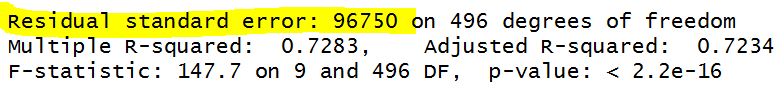
\includegraphics[width=4in]{std_err} \\
      \end{center}

    \end{frame}



    \begin{frame}{Again: regression assumptions}
      Remember the big four:
      \begin{enumerate}
        \item \alert{The residuals are independent.}
        \item $Y$ is a linear function of $X$s (except for the errors).
        \item The residuals are normally distributed.
        \item The variance of $Y$ is the same for any value of $X$s (``homoscedasticity'').

      \end{enumerate}
    \end{frame}


    \begin{frame}[fragile]{Assumption 1: Independence}
      Independence: No correlation between residuals \pause --- we have to think this through; can't use a plot here.
      \pause
      Remember that we want the \alert{cases} to be independent, not the \alert{variables}. We very much hope that $Y$ will be dependent on the $X$'s (otherwise, why are we trying to predict $Y$ based on the $X$'s?).
    \end{frame}





    \begin{frame}{Again: regression assumptions}
      Remember the big four:
      \begin{enumerate}
        \item The residuals are independent. \greencheckmark
        \item \alert{$Y$ is a linear function of $X$s (except for the errors).}
        \item The residuals are normally distributed.
        \item The variance of $Y$ is the same for any value of $X$s (``homoscedasticity'').
      \end{enumerate}
    \end{frame}



    \begin{frame}[fragile]{Assumption 2: Linearity}
      Plot the residuals vs the \alert{predicted Y-values} and ensure there is no trend:
\begin{knitrout}
\definecolor{shadecolor}{rgb}{0.137, 0.137, 0.137}\begin{kframe}
\begin{alltt}
\hlstd{> }\hlkwd{plot}\hlstd{(}\hlkwd{predict}\hlstd{(model),} \hlkwd{resid}\hlstd{(model),} \hlkwc{col}\hlstd{=}\hlstr{"green"}\hlstd{,}
\hlstd{+ }  \hlkwc{xlab}\hlstd{=}\hlstr{"Predicted values"}\hlstd{,} \hlkwc{ylab}\hlstd{=}\hlstr{"Residuals"}\hlstd{)}
\end{alltt}
\end{kframe}
\input{/tmp/figures/unnamed-chunk-9-1.tikz}

\end{knitrout}
    \end{frame}


    \begin{frame}{Again: regression assumptions}
      Remember the big four:
      \begin{enumerate}
        \item The residuals are independent. \greencheckmark
        \item $Y$ is a linear function of $X$s (except for the errors). \greencheckmark
        \item \alert{The residuals are normally distributed.}
        \item The variance of $Y$ is the same for any value of $X$s (``homoscedasticity'').
      \end{enumerate}
    \end{frame}



    \begin{frame}[fragile]{Assumption 3: Normally distributed residuals}
      Ensure that the Q-Q plot shows a (roughly) straight line:
\begin{knitrout}
\definecolor{shadecolor}{rgb}{0.137, 0.137, 0.137}\begin{kframe}
\begin{alltt}
\hlstd{> }\hlkwd{qqnorm}\hlstd{(}\hlkwd{resid}\hlstd{(model),} \hlkwc{main}\hlstd{=}\hlstr{''}\hlstd{)}
\end{alltt}
\end{kframe}
\input{/tmp/figures/unnamed-chunk-10-1.tikz}

\end{knitrout}
    \end{frame}


    \begin{frame}{Again: regression assumptions}
      Remember the big four:
      \begin{enumerate}
        \item The residuals are independent. \greencheckmark
        \item $Y$ is a linear function of $X$s (except for the errors). \greencheckmark
        \item The residuals are normally distributed. \greencheckmark
        \item \alert{The variance of $Y$ is the same for any value of $X$s (``homoscedasticity'').}
      \end{enumerate}
    \end{frame}


    \begin{frame}[fragile]{Assumption 4: The variance of $Y$ is the same across}
      Look for a (roughly) constant vertical ``thickness'':
\begin{knitrout}
\definecolor{shadecolor}{rgb}{0.137, 0.137, 0.137}\begin{kframe}
\begin{alltt}
\hlstd{> }\hlkwd{plot}\hlstd{(}\hlkwd{predict}\hlstd{(model),} \hlkwd{resid}\hlstd{(model),} \hlkwc{col}\hlstd{=}\hlstr{"green"}\hlstd{,}
\hlstd{+ }  \hlkwc{xlab}\hlstd{=}\hlstr{"Predicted values"}\hlstd{,} \hlkwc{ylab}\hlstd{=}\hlstr{"Residuals"}\hlstd{)}
\end{alltt}
\end{kframe}
\input{/tmp/figures/unnamed-chunk-11-1.tikz}

\end{knitrout}
    \end{frame}

    \begin{frame}{Again: regression assumptions}
      Remember the big four:
      \begin{enumerate}
        \item The residuals are independent. \greencheckmark
        \item $Y$ is a linear function of $X$s (except for the errors). \greencheckmark
        \item The residuals are normally distributed. \greencheckmark
        \item The variance of $Y$ is the same for any value of $X$s (``homoscedasticity'').  \greencheckmark
      \end{enumerate}
      \pause
      \alert{w00t w00t!} \pause This model meets the assumptions for regression, so it is safe to interpret $p$-values and confidence intervals.
      \lc
    \end{frame}


    \begin{frame}[fragile]{We have a model. Now what?}
      Let's make some predictions.
    \end{frame}


    \begin{frame}[fragile]{Making predictions}
      The regression model estimates the coefficients of the predictors:
      \fontsize{9}{9}\selectfont
\begin{knitrout}
\definecolor{shadecolor}{rgb}{0.137, 0.137, 0.137}\begin{kframe}
\begin{alltt}
\hlstd{> }\hlkwd{round}\hlstd{(}\hlkwd{summary}\hlstd{(model)}\hlopt{$}\hlstd{coefficients,} \hlnum{4}\hlstd{)}
\end{alltt}
\begin{verbatim}
                Estimate Std. Error  t value Pr(>|t|)
(Intercept)  840065.1500 99001.0317   8.4854    0e+00
CRIME         -2566.0842   663.8172  -3.8656    1e-04
ZONE            921.9981   276.2196   3.3379    9e-04
NOX         -346925.6722 71811.3231  -4.8311    0e+00
ROOM          74242.5198  8261.8840   8.9861    0e+00
DIST         -31049.5290  3784.9798  -8.2034    0e+00
RADIAL         6000.2426  1288.1421   4.6581    0e+00
TAX            -265.3307    68.5657  -3.8697    1e-04
PTRATIO      -19279.7516  2627.2042  -7.3385    0e+00
LSTAT        -11071.7310   957.4835 -11.5634    0e+00
\end{verbatim}
\end{kframe}
\end{knitrout}

    \end{frame}


    \begin{frame}[fragile]{Making predictions}
      Let's estimate the median house price in a particular district:
      \fontsize{9}{9}\selectfont

      \begin{table}[!b]
        {\carlitoTLF % Use monospaced lining figures
        \begin{tabularx}{\textwidth}{XXrrr}

           $j$ & Predictor  & $\beta_j$   &  $X_j$  & $\beta_j X_j$ \\
          \toprule
            0 & Intercept	&	840.07	&	1	&	840.07  \\
            1 & CRIME	&	-2.57	&	0.03	&	-0.0771  \\
            2 & ZONE	&	0.92	&	10	&	9.2  \\
            3 & NOX	&	-346.93	&	0.5	&	-173.465  \\
            4 & ROOM	&	74.24	&	4	&	296.96  \\
            5 & DIST	&	-31.05	&	5	&	-155.25  \\
            6 & RADIAL	&	6	&	1	&	6  \\
            7 & TAX	&	-0.27	&	300	&	-81  \\
            8 & PTRATIO	&	-19.28	&	15	&	-385.6  \\
            9 & LSTAT	&	-11.07	&	10	&	-110.7  \\
          \bottomrule
             Price &  Estimate 	& 	&		&	342.538   \\


        \end{tabularx}}

      \end{table}

    \end{frame}



    \begin{frame}[fragile]{Making predictions}
      Let R do it for us!

\begin{knitrout}
\definecolor{shadecolor}{rgb}{0.137, 0.137, 0.137}\begin{kframe}
\begin{alltt}
\hlstd{> }\hlkwd{predict.lm}\hlstd{(model,} \hlkwd{list}\hlstd{(}\hlkwc{CRIME}\hlstd{=}\hlnum{0.03}\hlstd{,} \hlkwc{ZONE}\hlstd{=}\hlnum{10}\hlstd{,}
\hlstd{+ }                       \hlkwc{NOX}\hlstd{=}\hlnum{0.5}\hlstd{,} \hlkwc{ROOM}\hlstd{=}\hlnum{4}\hlstd{,}
\hlstd{+ }                       \hlkwc{DIST}\hlstd{=}\hlnum{5}\hlstd{,}  \hlkwc{RADIAL}\hlstd{=}\hlnum{1}\hlstd{,}
\hlstd{+ }                       \hlkwc{TAX}\hlstd{=}\hlnum{300}\hlstd{,} \hlkwc{PTRATIO}\hlstd{=}\hlnum{15}\hlstd{,}
\hlstd{+ }                       \hlkwc{LSTAT}\hlstd{=}\hlnum{10}\hlstd{))}
\end{alltt}
\begin{verbatim}
       1 
343955.2 
\end{verbatim}
\end{kframe}
\end{knitrout}
      \note{The discrepancy is due to rounding in the previous slide.}

    \end{frame}


    \begin{frame}[fragile]{Model coefficients}
      Suppose there are 420 students and 28 teachers in the disctrict ($\text{PTRATIO}=420/28=15$). \pause

      \bigskip

      The school board is considering hiring 2 more teachers. How would this affect the house prices in the district? \pause

      \bigskip

      The new PTRATIO will be $420/30=14$. \pause

\begin{knitrout}
\definecolor{shadecolor}{rgb}{0.137, 0.137, 0.137}\begin{kframe}
\begin{alltt}
\hlstd{> }\hlkwd{predict.lm}\hlstd{(model,} \hlkwd{list}\hlstd{(}\hlkwc{CRIME}\hlstd{=}\hlnum{0.03}\hlstd{,} \hlkwc{ZONE}\hlstd{=}\hlnum{10}\hlstd{,}
\hlstd{+ }                       \hlkwc{NOX}\hlstd{=}\hlnum{0.5}\hlstd{,} \hlkwc{ROOM}\hlstd{=}\hlnum{4}\hlstd{,}
\hlstd{+ }                       \hlkwc{DIST}\hlstd{=}\hlnum{5}\hlstd{,}  \hlkwc{RADIAL}\hlstd{=}\hlnum{1}\hlstd{,}
\hlstd{+ }                       \hlkwc{TAX}\hlstd{=}\hlnum{300}\hlstd{,} \hlkwc{PTRATIO}\hlstd{=}\hlnum{14}\hlstd{,}
\hlstd{+ }                       \hlkwc{LSTAT}\hlstd{=}\hlnum{10}\hlstd{))}
\end{alltt}
\begin{verbatim}
       1 
363234.9 
\end{verbatim}
\end{kframe}
\end{knitrout}
    \end{frame}



    \begin{frame}[fragile]{Model coefficients}
      To be able to compansate the new hires, the school district must add \$50 more on your tax bill for every \$10K of your house price. \pause

      \bigskip
      So, the tax rate increases to \$50 per \$10K. How would this affect the median house price?

      \lc

    \end{frame}



    \begin{frame}[fragile]{Confidence intervals}
      We know our predictions are not exactly right.

      Can we come up with some confidence intervals on our predictions? \pause
      \bigskip

      Remember the two kinds of intervals:
      \bigskip

      \begin{tabular}{lp{1in}p{2in}}
        \textbf{Confidence} & Predicting the mean value of $Y$ for a particular  set of $X$ values. & Among all the districts whose predictors are as above, what is the mean value of median house price?  \\
        \textbf{Prediction} & Predicting $Y$ for a single new case. & If Springfield has the predictors above, what is the median house price in Springfield?\\
      \end{tabular}


    \end{frame}



    \begin{frame}[fragile]{Confidence intervals}
\begin{knitrout}
\definecolor{shadecolor}{rgb}{0.137, 0.137, 0.137}\begin{kframe}
\begin{alltt}
\hlstd{> }\hlkwd{predict.lm}\hlstd{(model,} \hlkwd{list}\hlstd{(}\hlkwc{CRIME}\hlstd{=}\hlnum{0.03}\hlstd{,} \hlkwc{ZONE}\hlstd{=}\hlnum{10}\hlstd{,}
\hlstd{+ }                       \hlkwc{NOX}\hlstd{=}\hlnum{0.5}\hlstd{,} \hlkwc{ROOM}\hlstd{=}\hlnum{4}\hlstd{,}
\hlstd{+ }                       \hlkwc{DIST}\hlstd{=}\hlnum{5}\hlstd{,}  \hlkwc{RADIAL}\hlstd{=}\hlnum{1}\hlstd{,}
\hlstd{+ }                       \hlkwc{TAX}\hlstd{=}\hlnum{350}\hlstd{,} \hlkwc{PTRATIO}\hlstd{=}\hlnum{14}\hlstd{,}
\hlstd{+ }                       \hlkwc{LSTAT}\hlstd{=}\hlnum{10}\hlstd{),}
\hlstd{+ }                       \hlkwc{interval} \hlstd{=} \hlstr{'confidence'}\hlstd{)}
\end{alltt}
\begin{verbatim}
       fit      lwr      upr
1 349968.4 301948.5 397988.3
\end{verbatim}
\end{kframe}
\end{knitrout}
     \lc
     \end{frame}



     \begin{frame}[fragile]%{Confidence intervals}
        We can also put a confidence interval on a coefficient to estimate the plausible range of its effect.

        \fontsize{9}{9}\selectfont

\begin{knitrout}
\definecolor{shadecolor}{rgb}{0.137, 0.137, 0.137}\begin{kframe}
\begin{alltt}
\hlstd{> }\hlkwd{confint}\hlstd{(model)}
\end{alltt}
\begin{verbatim}
                   2.5 %       97.5 %
(Intercept)  645552.0530 1034578.2470
CRIME         -3870.3245   -1261.8439
ZONE            379.2933    1464.7029
NOX         -488017.5640 -205833.7804
ROOM          58009.9148   90475.1248
DIST         -38486.0994  -23612.9585
RADIAL         3469.3548    8531.1305
TAX            -400.0457    -130.6157
PTRATIO      -24441.5728  -14117.9304
LSTAT        -12952.9546   -9190.5075
\end{verbatim}
\end{kframe}
\end{knitrout}

        \fontsize{11}{13}\selectfont

        \pause
        We are 95\% confident that the effect of reducing the pupil/teacher ratio (PTRATIO) by 1 on median house price is between \$14K and \$24K!

        \lc
     \end{frame}



  \end{darkframes}

\end{document}
